\chapter{CSS}

\section{What is CSS}

Cascading Style Sheets (CSS) is a language for specifying how documents are presented to users.

A document is a collection of information that is structured using a markup language.

Presenting a document to a user means converting it into a useable form for your audience.

\begin{HTML5}[demo]
<!DOCTYPE html>
<html>
  <head>
  <meta charset="UTF-8">
  <title>Sample document</title>
  </head>

  <body>
    <p>
      <strong>C</strong>ascading
      <strong>S</strong>tyle
      <strong>S</strong>heets
    </p>
  </body>
</html>
\end{HTML5}

\section{Why use CSS}

Keeping the styles separate from your HTML content:
\begin{itemize}
\item Helps avoid duplication
\item Makes maintenance easier
\item Allows you to make a site-wide change in one place
\end{itemize}


\begin{CSS}[style1.css]
strong {color:red;}
\end{CSS}

\begin{HTML5}
<!DOCTYPE html>
<html>
  <head>
  <meta charset="UTF-8">
  <title>Sample document</title>
  <link rel="stylesheet" type="text/css" href="style1.css">
  </head>

  <body>
    <p>
      <strong>C</strong>ascading
      <strong>S</strong>tyle
      <strong>S</strong>heets
    </p>
  </body>
</html>
\end{HTML5}

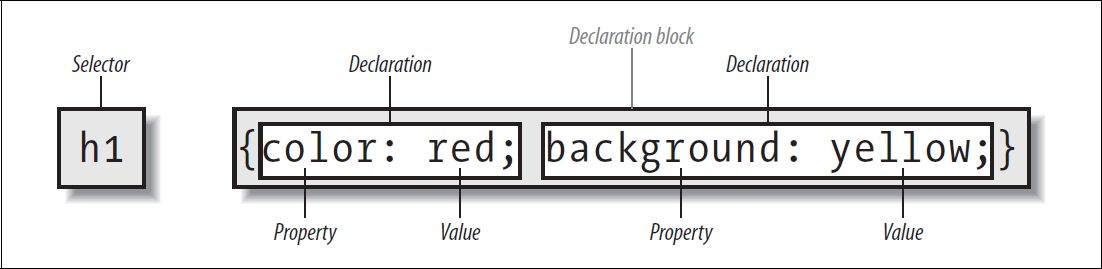
\includegraphics[scale=0.75]{css/resources/css-rule.jpg}

\section{Selector}

A selector is a chain of one or more sequences of simple selectors separated by combinators.

A sequence of simple selectors is a chain of simple selectors that are not separated by a combinator.



选择器是通过combinator分割开的一系列选择器组合起来的。

而一系列选择器是一系列简单选择器他们之间没有被combinator分开。

简单选择器是一个type selector, universal selector, attribute selector, class selector, ID selector, content selector, pseudo class。 而一个pesudo element可能出现在简单选择器的最后(???这个时候是简单选择器,还是一系列选择器??)。


\subsection{Simple selector}

A simple selector is either a type selector, universal selector, attribute selector, class selector, ID selector, content selector, or pseudo-class. One pseudo-element may be appended to the last sequence of simple selectors.

\subsubsection{Type selector}

A type selector is the name of a document language element type.

就是HTML的标签名来选择元素。

\begin{CSS}
<style>
p {color:red;}
div {border:1px; border-style:solid;}
</style>

<p>first line</p>
<p>second line</p>
<div>third line</div>
\end{CSS}


\subsubsection{Universal Selector}



\subsection{规则应用}

如果有多条规则应用到同一个元素,那么哪条规则会最终取胜。CSS提供了三种机制:继承,层叠和特指。


\subsubsection{继承}

从祖先元素继承样式;CSS中很多属性是可以继承的,相当一部分和文本相关,如颜色,字体,字号。

也有很多属性是不能继承的(因为继承这些属性没有意义)。不能继承的主要是涉及到元素盒子的定位和显示方式。比如边框,外边距,内边距。

\subsubsection{层叠}

对于元素中某个标签的特定属性值有多个来源是,最终确定使用哪个值。

Style sheets may have three different origins: author, user, and user agent.

样式来源主要有三个,浏览器,用户和作者:
\begin{itemize}
\item 第一,首先浏览器有个默认的样式表;
\item 然后,有一个用户样式表,可以通过用户样式表,来强制所有网站按这个样式来显示;
\item 在这就是作者样式表,有三种方式:连接样式,嵌入样式和行内样式
\end{itemize}

层叠顺序
\begin{enumerate}
\item 浏览器默认样式表
\item 用户样式表
\item 作者连接样式表(按照特闷连接到页面的先后顺序)
\item 作者嵌入样式
\item 作者行内样式
\end{enumerate}

按上面的顺序来更新对每个标签属性的值,这个检查结束后,再将每个标签以最终设定的样式显示出来。


最终的层叠规则是:
\begin{enumerate}
\item 先找出每个元素以及元素的属性;
\item 按照顺序和权重排序,顺序就是上述五个来源来选择,权重可以通过\lstinline$空格!important$来加重声明的权重。
\item 按特指读排序。表示一条规则有多明确,则优先级别高
特制度计算:I-C-E
\begin{itemize}
\item 选择符中有一个ID,就在I的位置上加1;
\item 选择符中有一个类,就在C的位置上加1;
\item 选择符上有一个元素标签名,就在E的位置加上1;
\end{itemize}
\item 如果所有都一样,则声明靠后的优先级别高
\end{enumerate}


\section{属性}

属性值主要分为三类:

\begin{itemize}
\item 文本值
\item 数字值,数字值分为绝对值和相对值;

绝对值这里我们只使用像素(px);

相对值有(em, ex, \%),em表示一种字体中字母"M"的宽度,ex等于字体中字母"x"高度。\%百分比适合设定诶包含的元素的宽度。

\item 颜色值,颜色名(red),16进制颜色(\#RGB,\#RRGGBB),RGB颜色值(rgb(0,255,0)),RGB百分比值(R\%,G\%,B\%),HSL(色相,饱和度\%,亮度\%)
\end{itemize}


\section{定位元素}

盒模型就是页面中的每个元素生成的矩形盒子。这些合资都要按照课件板式模型在页面上排布。主要由三个属性控制:position,display,float。

其中,position属性控制页面上元素间的位置关系;display控制元素是堆叠,还是并排,还是根本不在页面上出现;float属性提供控制的方式,以便把元素组成多栏布局(???这个解释不是太清楚)。

\subsection{盒模型}

盒子的属性:
\begin{itemize}
\item 边框(border),可以设置边框的宽窄,样式和颜色;
\item 内边距(padding),可以设置盒子内容区域边框的间距;
\item 外边距(margin),可以设置盒子与相邻元素的间距。
\end{itemize}

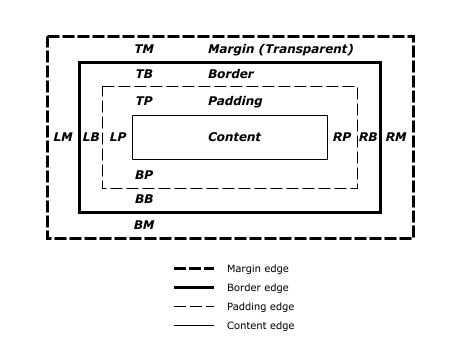
\includegraphics[scale=1]{css/resources/box-mode.png}


\begin{CSS}[上 右 下 左]
{margin: 5px 10px 12px 18px;}
\end{CSS}

如果有值没有写,则取对边的值,如果只写了一个值,则四边都取这个值。


border三个属性 宽度(width), 样式(style), 颜色(color)。 border还有第四个属性radius,但是不影响和模型的定位。

\begin{CSS}[三个粒度]
{border: 2px dashed red;} // 全部3个属性,全部4条边
{border-style: dashed;} // 一个属性,四条边
{broder-left-style: dashed;} // 一个属性,一条边
\end{CSS}

内边框和外边框。


\begin{CSS}[中和外边框和内边框,使不同浏览器效果一致]
* {margin: 0; padding: 0;}
\end{CSS}


(!!!!我记得这和有个什么显示方式有关,默认情况下上下排列才是垂直方向上外边距叠加,需要看文档补充一下)
垂直方向上的外边距会叠加。

外边框叠加,比如有两个段落,第1个段落的下外边距是50px,第2个段落的上外边框为30px,那么他们之间的外边框是50px。因为这种上下外边框相遇的情况下,他们会相互重叠,直到一个外边框碰到另一个元素的边框。

\subsubsection{盒子大小}

对于块级元素,如果没有设置width,那么他的默认值就是auto,结果会让元素的狂度扩充到与父元素同宽;如果添加水平边框,内边距和外边距,会导致内容宽度减少,减少量等于水平边框,内边距和外边距增加之和。

明确设定width之后,块级元素就不会再扩展到与父元素同宽了。盒子width属性指定的只是盒子内容区的宽度,而不是盒子要占住的水平宽度。


\subsection{float \& clear}

